My educational journey was profoundly shaped by the dedication and expertise of several remarkable teachers and mentors, who have led me to believe in the transformative power of good teaching on a student's life trajectory. This belief is reinforced by today's abundance of high-quality, open online courses from top universities, which provide nearly identical technical content to their in-classroom counterparts. This democratization of higher education has emphasized the importance of an instructor's role in guiding students through the learning process, rather than simply delivering information. As cliché as it may sound, what still remains true as a teaching philosophy is to teach students \emph{how} to think, rather than \emph{what} to think. With the increasingly diversified student body and teaching modality, both of which important for expanding the accessibility of higher education, it also requires a more nuanced approach to balance the act of engaging, conveying, and inspiring. To implement this philosophy into pedagogical practice, I am often guided by a series of introspective questions that aims to ensure that my lecture content is not only informative but also stimulating for critical thinking:
\begin{quote}
    \begin{enumerate}[nosep,leftmargin=*]
        \item What can students take away from actively engaging with my lecture?
        \item What can students take away from the slides displayed in-classroom?
        \item What can students take away from revisiting the slides on their own pace?
        \item How can I ensure consistency in these takeaways gathered across varied learning contexts?
        \item How do I structure the content to convey key messages to students without them directly reading from it?
    \end{enumerate}
\end{quote}

\section*{Teaching Philosophy}

To answer these questions, I draw from my personal experience\textemdash{}having worked over the years with people that can fall into two almost distinct categories: \emph{device physicists} and \emph{system engineers}. The former often approach problems from first principles to find solutions, sometimes simplified, in an elegant and analytical way, while the latter often emphasize the efficiency of an algorithmic approach, even if the algorithm itself can sometimes be a black box. The two groups of minds apparently have worked well together in creating some of the most advanced technological wonders\textemdash{}think of building a supercomputer from sand\textemdash{}the underlying approach to problem-solving is what I find most appreciable. By leveraging the benefits from both worlds using a ``pragmatic first principles'' approach which first identifies the malleable parts of nature before proceeding to a solution. While engineering inherently requires a high degree of abstraction and consideration of practical constraints, understanding limitations at their most fundamental physical level provides invaluable insight and forms the essential foundation of a highly effective problem-solving framework. Given the highly interdisciplinary curriculum at \appSchoolDeptShort{}, I believe this philosophy and general approach to teaching will transfer seamlessly to my efforts as an instructor and enrich students' preparedness for solving the nuanced challenges of real-world science and engineering problems.

I additionally value the role of good-quality visualization for improving teaching effectiveness, leveraging human brain's rapid image processing ability, which reportedly surpasses text interpretation by 6x\textendash 600x\footnote{
    Despite the discrepancy with the unfounded internet meme claiming 60,000x, as called out in \emph{The 60,000 Fallacy} (\url{https://policyviz.com/2015/09/17/the-60000-fallacy/}), this is still substantial enough to warrant extra attention to the use of visualization in teaching.
}~\cite{ResearchPictureWorth}. This capability enables students to extract information from visual aids alongside verbal explanations far more efficiently than text alone, allowing for profound engagement in class. In the realm of STEM education, where abstract theories and complex equations can be overwhelming, visualization serves as a vital bridge, translating intricate ideas into comprehensible and memorable images. It also elegantly addresses the pedagogical challenge of conveying essential concepts without resorting to simply reading from the slides\textemdash a practice that hinders critical thinking. Beyond the immediate classroom benefits, the ability to visualize data and concepts is an indispensable skill for students, one that is increasingly critical in both their academic pursuits and future research careers. Building on this philosophy, I address the challenge of ensuring consistent takeaways from the course materials in different learning contexts\textemdash whether inside or outside the classroom\textemdash by integrating concise bullet points alongside visuals, ensuring key messages being conveyed.

\section*{Teaching Experience}
Beginning early on during my time as a graduate student, I sought out opportunities to get involved with teaching and tutoring. I was a teaching assistant for multiple undergraduate-level courses encompassing both lecture-based and lab-based formats. As a teaching assistant for the course ``ECE 153B: Sensor \& Peripheral Interface Design'' at \myPhDSchoolShort{}, I led quality lab sessions and office hours to help students navigate through the hardware and software debugging challenges, ensuring each and every student had an original and successful final project demonstration. Throughout this experience, I gained firsthand insight on how to balance the time and attention allocated to each student with different progress levels\textemdash{}some students at faster pace might encounter more advanced issues that require longer time to resolve, yet this must be done without compromising the learning experience of students that need more guidance on the basics. The most rewarding part of this experience was witnessing the demonstrations of various hardware projects, which emerged from brainstorming with students and guiding them through a few months of iterative design and debugging. I received several emails from the students even after the semester ended, expressing their gratitude for the guidance and mentorship, without which they would not have been able to complete the project.

\begin{wrapfigure}{r}{0.45\textwidth}
    \vspace{-1em}
    \begin{center}
        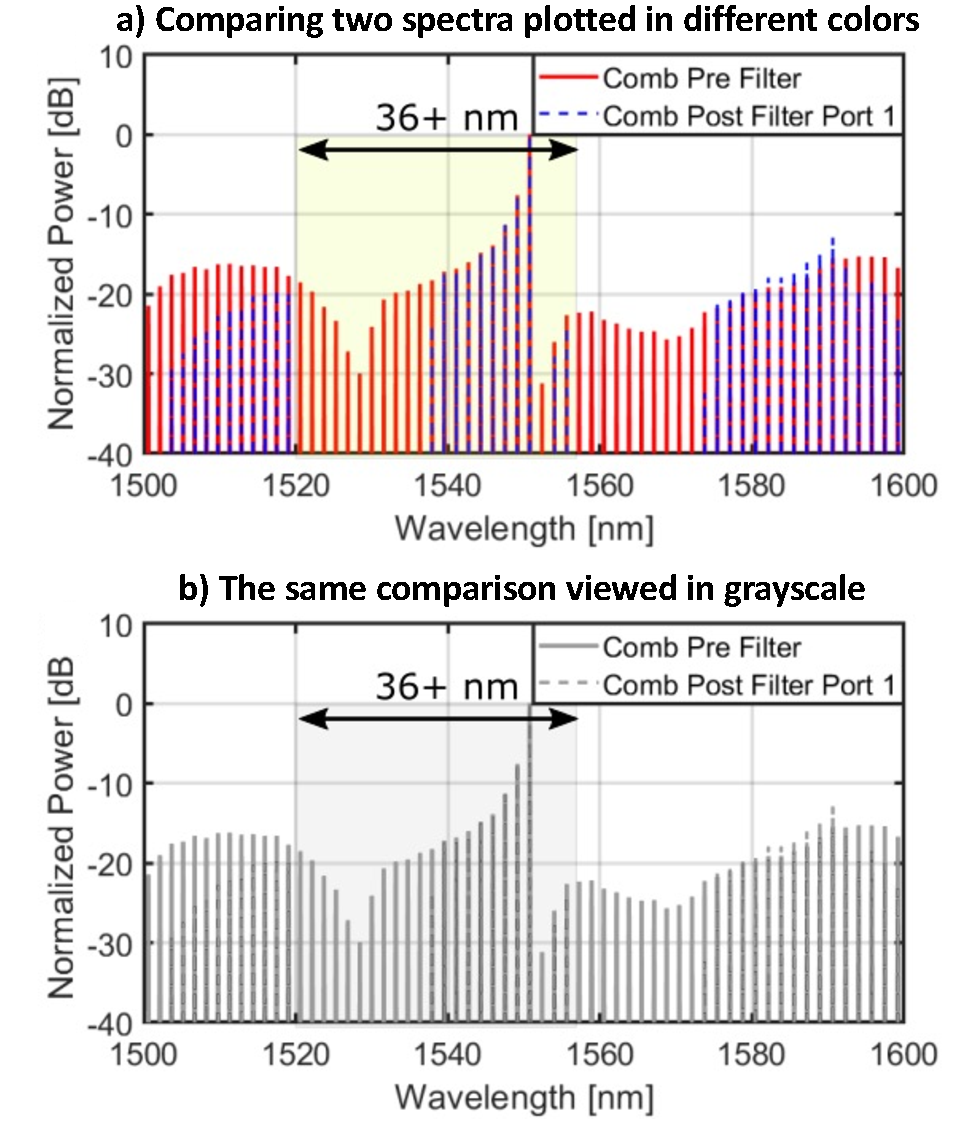
\includegraphics[width=\linewidth]{../../6_figures/ts_fig_color.pdf}
    \end{center}
    \caption{Example of non-robust information encoding solely with color contrast. (a)~Two spectra distinguishable by people with normal color vision. (b)~Illustrative rendering of the same two spectra possibly perceived by people with color vision deficiency.}
    \label{fig:color}
    \vspace{-0.5em}
\end{wrapfigure}

I have also shared my personal experience and lessons learned in preparing and presenting visual content with the graduate students at \mySchoolShort{}. Designing visuals that effectively encode information demands thoughtful consideration and attention to detail, ensuring accessibility for all learners. Informed by my personal experience with minor color vision deficiency, I am acutely aware of key pitfalls in visual information delivery, such as solely relying on color contrast to embed information. The prevalence of color blindness, affecting approximately 8\% of males and 0.5\% of females~\cite{TypesColourBlindness}, might surprise many. However, this statistic virtually guarantees that in any moderately sized classroom, at least one individual is likely to have a form of color vision deficiency. In a lecture titled ``Color Blindness\textendash{}Aware Scientific Visualization for Robust Information Conveyance'', I showed Fig.~\ref{fig:color} as an example to demonstrate how using color as the sole differentiator between two spectra can make the data difficult to interpret for those with color vision impairments. This lecture was very well received as some students were surprised by their unawareness of the issue yet the simple solutions that can be implemented to make the visual content more accessible. This experience has always reminded my of what an instructor can offer beyond the technical content. My commitment to inclusivity also extends beyond this to embrace all facets of diversity and accessibility in education. I recognize that students come with a broad spectrum of cultural backgrounds, personal histories, and educational experiences, all of which influence their learning needs. In light of this, I will strive to create a classroom environment that is not only physically accessible but also cognitively and culturally welcoming. This entails the use of language that is inclusive and bias-free, as well as the incorporation of diverse examples in my teaching materials, practices that I will regularly reflect on to ensure adherence.

During my senior \myDegree{} and postdoc time, I have also taken on significant leadership roles for many of our major research projects—these roles often required diffuse mentorship across large collaborative efforts in addition to highly focused, fast-paced teaching aimed at quickly bringing new students up to speed. To me, mentoring extends beyond knowledge sharing and intellectual guidance, and further involves providing holistic support for
the academic and professional development of the students. Through the mentoring of more than ten graduate and undergraduate students at \mySchoolShort{}, I partially put this philosophy into practice and guided several Ph.D. students to significant milestones, including publishing their first papers as lead authors and securing their initial industry positions. I believe these essential skills built from my broad experience as a mentor will enable a
smooth transition to training highly successful students as a teacher and a principal investigator. I eagerly anticipate the opportunity to extend and refine my teaching and mentoring practices at \appSchoolDeptShort{}.

\section*{Teaching Plan}
At \appSchoolShort{}, I plan to leverage the lessons learned through trial and error from my previous years of teaching experience and pragmatically test new ideas from statistically-backed contemporary literature~\cite{deslauriersMeasuringActualLearning2019,bathgatePerceivedSupportsEvidencebased2019} in order to provide an environment which fosters maximal growth across all students, independent of background and learning style. I am both prepared and qualified to teach undergraduate/graduate
courses in focused areas such as \emph{integrated photonics}, \emph{optical interconnects}, and \emph{electronic-photonic design automation}, as well as core courses in electrical and computer engineering such as \emph{semiconductor devices}, and \emph{digital logic design}. Believing that the preparation for teaching materials deepens my own understanding of the subject matter, I am also open to teaching courses beyond my immediate expertise, such as \emph{computer architecture}.